\section{Design and Implementation}
\label{sec:DesignImplementation}
\subsection{Algorithmic Design}
\label{sec:AlgorithmicDesign}
\subsubsection{Definitions}
\label{sec:Definitions}
A \textit{frame} is a two-dimensional array of pixels and a \textit{video} is a sequence of frames. Depending on the type of video, the frames may be grayscale (in which case each pixel contains a single scalar value) or color (in which case pixels contain multiple values that represent color channels). A video can be indexed with a particular index $i$ to retrieve the $i^{th}$ frame as long as $i$ is less than $l$, the total number of frames in the video. 
An \textit{approximate frame} $f'$ is a frame derived from another frame $f$. $f'$'s pixel values are related to $f$'s pixel values according to some function. Depending on the function, $f'$ may contain less or as much information as $f$. As the name implies, however, it is often the case that $f’$ contains less information than f. 
Let $D$ be a function that takes an input video $v$ and two indexes $x$ and $y$ and returns a scalar result. The result of $D(v, x,y)$ is the distance between the frames $x$ and $y$ in the video $v$. There are many different possible ways to define $D$ and calculate the distance. Our definition is based on Euclidean distance and outlined below in detail.
We define a \textit{video sequence} as a pair of indices $(x,y)$ where $x$ is greater than $y$ and $x$ and $y$ are less than $l$. A video sequence $(x,y)$ for video $v$ is \textit{well-looping} if $D(v,x,y) < T$ where $T$ is a threshold value. A \textit{video loop} is a well-looping video sequence $(x,y)$ for video $v$.
\subsubsection{Distance}
\label{sec:Distance}
The distance metric used in our approach is based on the Euclidean distance. It is as follows:
$$d(F_1,  F_2) = \sqrt{\sum_{i=1}^N (F_1[i] -  F_2[i])^2}.$$
Note that the above metric is for intensity images. The core idea still applies to full color images; the internal subtraction is just done in each color channel. 

This distance metric is simple enough to implement: the full color version is shown in pseudocode below.
\begin{verbatim}
def d(im1, im2):
  i1_s = im1.shape
  i2_s = im2.shape
  distance = 0
   for x in range(i1_s[0]):
    for y in range(i1_s[1]):
     for z in range(i1_s[2]):
      if im1[x][y][z] == im2[x][y][z]:
       continue
      distance += abs(im1[x][y][z] 
       - im1[x][y][z])**2
     return (distance /
       (i1_s[0] * i1_s[1] * i1_s[2]))**(1/2)
\end{verbatim}
Despite its simplicity, most of our distance calculations do not follow this implementation. We rewrite it in a mathematically equivalent way, according to the law of consines. The above equation can be reformed into the following:
																																														$$d(F_1,  F_2) = \sqrt{ \|F_1\|_2^2 + \| F_2\|_2^2 - 2 (F_1 \cdot  F_2) }$$
																																														where the notations are used
																																														$$\|F\|_2^2 = \sum_{i=1}^N F[i]^2,  \,\,\,\,\,\,\, F_1 \cdot F_2 =  \sum_{i=1}^N F_1[i]F_2[i]$$
																																														This form of the distance equation performs the same as the original, but has an added benefit: because $\|F\|_2^2$ depends only on a single frame (and not a pair of frames), it can be precomputed. This leaves the actual distance formula with fewer calculations. The original had approximately $3N$ calculations: $N$ subtractions, $N$ multiplications, and $N-1$ additions. The new distance formula, with the norms precomputed only requires $2N$ calculations, resulting in an overall speedup. 
\subsubsection{Masks}
\label{sec:Masks}
Masks can be used to filter or replace pixel values in the frames of a video \cite{Piccardi2004}. For example, a mask can filter out all the blue in the frames of a video or replace all pixels outside a particular region with pixels from an external image. A mask might also indicate the region of frames where interesting motion exists throughout a video. 
In the scope of this project, we define the mask as a single two-dimensional array with the same height and width as the frames of the video. The mask may also have associated data (used to make filtering decisions, define replace values, etc). 
Masks can serve two purposes in building video loops: functional and aesthetic. Functionally, masks may help the loop detection algorithm stabilize a shaky input video. A mask could define the moving parts of the video and build approximate frames from that subregion. A user could define a mask as a hint to the loop detection algorithm. We did not implement functional masks in the current version of the system.
Aesthetic masks affect the look of the video produced by the system. For example, they could be used to define the regions of the frames that should be replaced with a solid color or cropped out entirely. We implemented two different aesthetic masks: colorize and background. The colorize mask is used to define a region of pixels of a frame that should retain their original color values -- pixels outside the region will be converted to grayscale. The background mask defines a region of pixels of a frame that should be replaced with pixel values from some external image. 
In the system, masks can be defined according to the median and mean values of a pixel across a video. Masks are applied to frames depending on the difference between the actual value of a pixel and the median (mean) value of that pixel throughout the video. As mentioned above, each mask defines a way to alter the pixel value when the difference exceeds the threshold. 
\subsubsection{Pipeline}
\label{sec:Pipeline}
\begin{figure*}
\centering
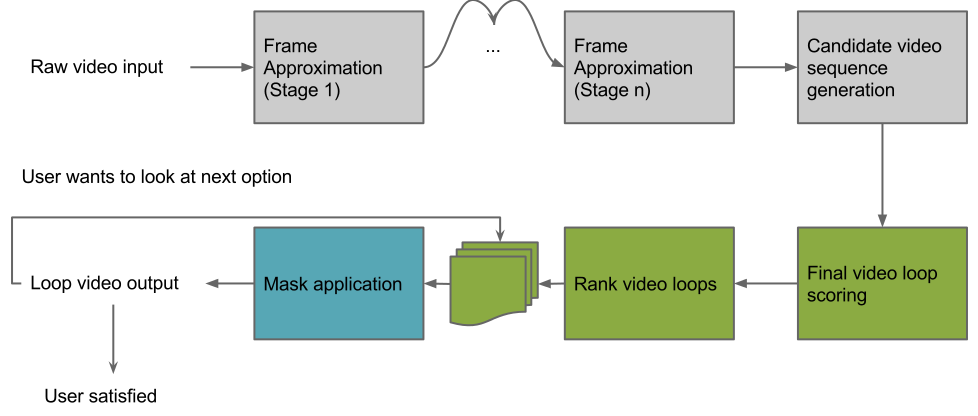
\includegraphics[width=1.0\textwidth]{loop-pipeline.png}
\caption{Overall workflow of UpvoteetovpU}
\label{fig:Pipeline}
\end{figure*}
The final pipeline for our approach is as follows: first, user parameters are read and their effects are implemented. The possible parameters are shown by example:
\begin{itemize}
\item \textbf{-o all} : Performs optimization based on edges and downsampling
\item \textbf{-l 1s -m 7s} : Restricts the output length to be between 1 second and 7 seconds. If parameters do not include the `s', they will be treated as frame counts
\item \textbf{-s 100 -e 250} : Restricts the algorithm's search space to starting at the $100^{th}$ line and ending at the $250^{th}$ line
\item \textbf{-t 20} : sets the threshold for determining which frame pairs are testing in full colorspace (is meaningless if no optimization is used)
\item \textbf{-i} : Runs in interactive mode, allowing user to see more than just the single best output
\end{itemize}

With these parameters set, the next step in the pipeline is to create the relevant \texttt{Video} objects (see Section~\ref{sec:Video}). If the user has opted to compute any approximations for an optimization (such as edge frames or scaled frames), those are computed. Then, the approximation is run through a function that computes the distance between all relevant pairs of frames (see Section~\ref{sec:Distance}). It returns a list of frame pairs and distances that is then sorted for distance. All of the candidate pairs from the approximations that have a distance below the set threshold are run through the full color distance function. Those results are also sorted for distance. Then, the best frame pair for creating a perfect loop is the first item in the sorted list. Before the results are presented to the user, a mask may be applied for aesthetic purposes (see Section~\ref{sec:Masks}). In regular mode, a GIF is created with those endpoints. In interactive mode, the user can opt to get the next-best result if the current one is not desirable.

\subsection{Implementation Design}
\label{sec:ImplementationDesign}
The system is implemented in Python and uses a set of external libraries. The system relies on NumPy \cite{NumPy}, OpenCV \cite{OpenCV}, and skimage \cite{skimage}. In the following sections, we describe, at a high level, the implementation of the system.
\subsubsection{Video}
\label{sec:Video}
A \textit{video} is implemented as a \texttt{Video} object. Each video object has certain properties (like the name of the source video file if it was created from a file stored on disk, the total number of frames, etc) and certain methods. 
The frames of the video are stored as an array within the video object. Each frame of a video is accessible through the \texttt{[i]} operator where $i$ is the frame index. The result of the \texttt{[i]} operation is a frame -- a two-dimensional array whose individual objects are formatted according to the type of video. The \texttt{[i:j]} operator, where $i$ and $j$ are frame indexes and $j>i$, creates a new \texttt{Video} whose contents are the frames from $i$ to $j$, inclusive. 
A \texttt{Video} knows how to turn itself into an animated GIF and store the output into a file. A video also knows how to iterate through itself in an idiomatic Python way. 
There are three subclasses of \texttt{Video} (\texttt{GrayVideo}, \texttt{EdgeVideo} and \texttt{ScaleVideo}) that can be instantiated from existing \texttt{Video} objects or from videos stored in files on disk. When a \texttt{GrayVideo} is instantiated, the frames are immediately converted to grayscale. When an \texttt{EdgeVideo} is instantiated, its frames are immediately run through a Canny edge detector. When a \texttt{ScaleVideo} is instantiated, its frames are immediately scaled to a new size. By instantiating one of these subclasses from an existing \texttt{Video} object, a video of approximate frames is immediately available. It is possible to ``chain'' instantiations so that the approximations can be applied one-after-another. 
\subsubsection{Mask}
\label{sec:Mask}
A \textit{mask} is implemented as a \texttt{Mask} object. Each mask object has certain properties (like a threshold value) and certain methods and requires at least a \texttt{Video} object \textit{v} as a parameter for construction. The frames of \textit{v} determine the values of the mask depending on the type of mask. These mask values are stored as a two-dimensional array within the object. A mask value at pixel $(i,j)$ is accessible by indexing a mask object using \texttt{[i][j]}. 
A \texttt{Mask} implements a \texttt{decide} function. \texttt{decide} takes three parameters (frame index, pixel location and existing value of the pixel). The function returns an updated value to be stored in that location. It may simply return the existing value if it does not want to change the value. 
We implement two \texttt{Mask} subclasses: \texttt{MedianMaskBackground} and \texttt{MedianMaskColorize}. Each of these calculates mask values based on the median of pixel values throughout the video. 
Besides a \textit{Video}, the \texttt{MedianMaskBackground} takes an image \textit{i} as a parameter for construction. \textit{i} must have the same shape as the frames of \textit{v}. The \texttt{decide} function of a \texttt{MedianMaskBackground} replaces a frame's pixel with the equivalent pixel from \textit{i} when it differs by more than the mask's threshold.
The \texttt{decide} function of a \texttt{MedianMaskColorize} replaces a frame's pixel with the grayscale equivalent when it differs by more than the mask's threshold.
